
\begin{figure}
\centering
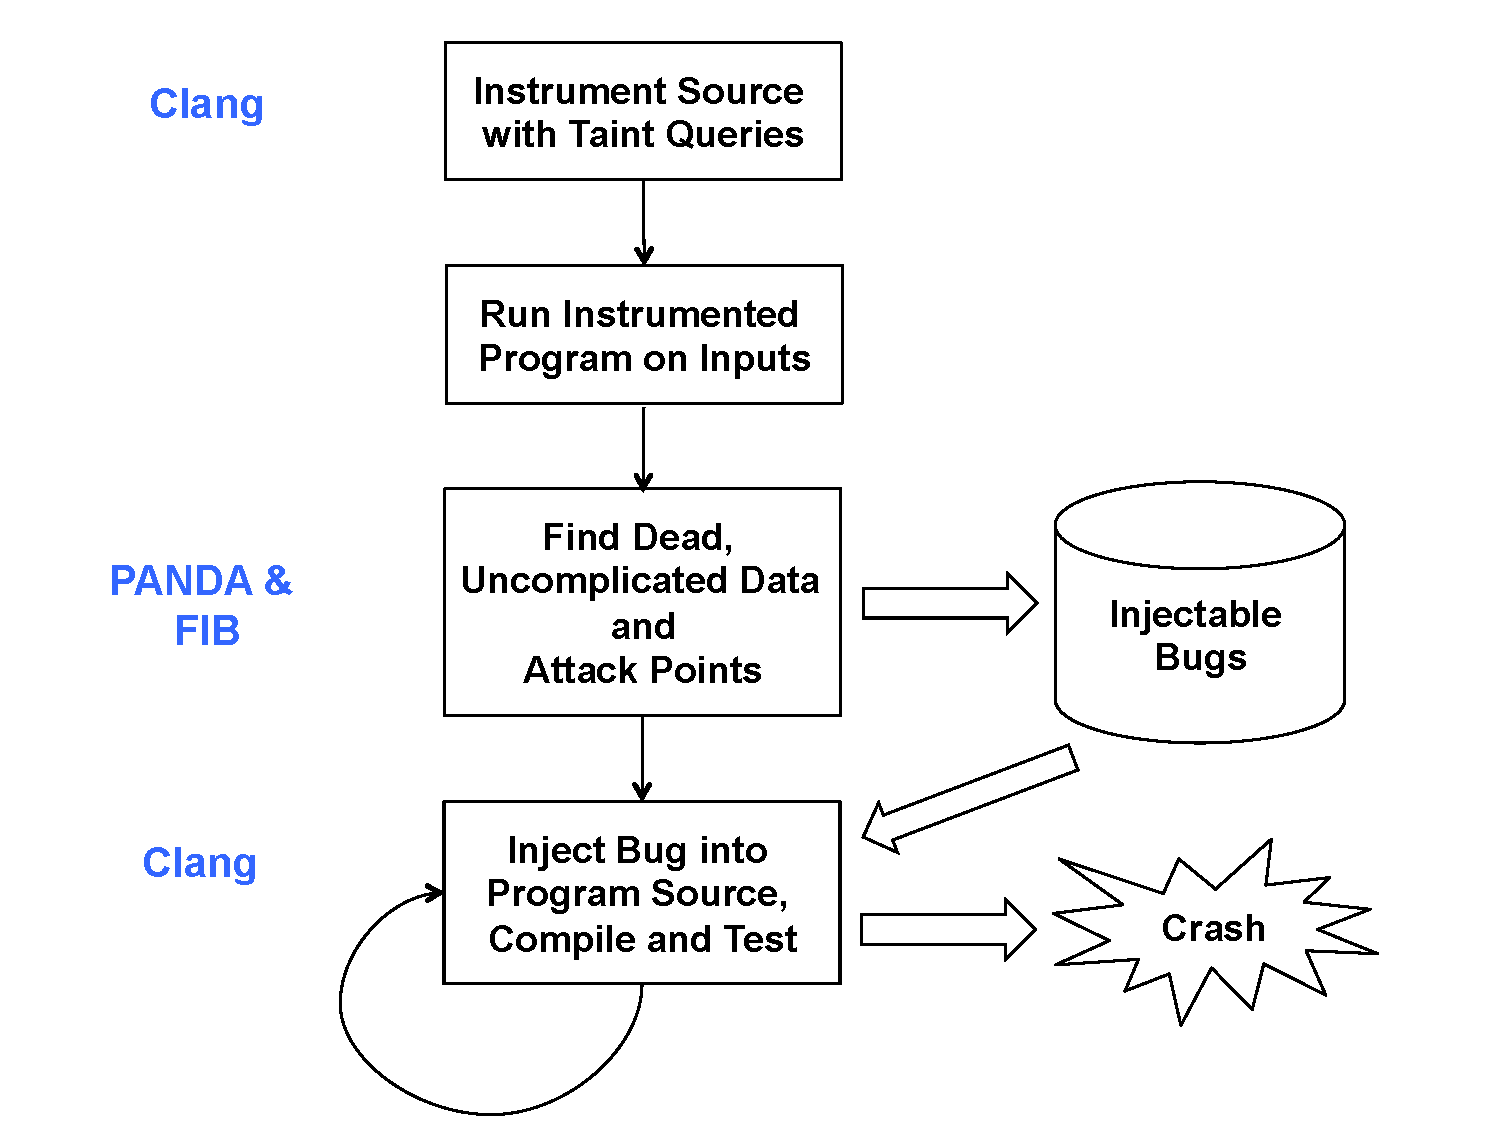
\includegraphics[width=3.5in]{lava-arch.pdf}
\caption{LAVA Implementation Architecture.  PANDA and Clang  are used to perform a dynamic taint analysis which identifies potential bug injections as DUA attack point pairs.
Each of these is validated with a corresponding source code change performed by Clang  as well.
Finally, every potentially buggy binary is tested against a targeted input change to determine if a buffer overflow actually results.}
\label{fig:lava-impl}
\end{figure}

\todo[inline]{Ricky: captions for figures should be smaller font, or something different. In some places it is hard to visually tell the figure caption from the text of the paper. see fig ~\ref{fig:lava-impl}, fig:lava-impl}


The LAVA implementation operates in four stages to inject and validate buffer overflow vulnerabilities in Linux C source code. 

\begin{enumerate}
\item Compile a version of the target program which has been instrumented with taint queries.
\item Run the instrumented version against various inputs, tracking taint, and collecting taint query results and attack point information.
\item Mine the taint results for DUAs and attack points, and collect a list of potential injectable bugs.
\item Recompile the target with the relevant source code modifications for a bug, and test to see if it was successfully injected.
\end{enumerate}

These stages are also depicted in Figure~\ref{fig:lava-impl}.

\subsection{Taint queries}
LAVA's taint queries rely on the PANDA dynamic analysis platform~\cite{PANDA}, which is based on the QEMU whole-system emulator.
PANDA augments QEMU in three important ways.
First, it introduces deterministic record and replay, which can be used for iterated and expensive analyses that cannot be performed online.
Second, it has a simple but powerful plugin architecture that allows for powerful analyses to be built and even built upon one another.
Third, it integrates, from S2E~\cite{S2E}, the ability to lift QEMU's intermediate language to LLVM for analysis.

The main feature of PANDA used by LAVA is a fast and robust dynamic taint analysis plugin that works upon the LLVM version of each 
basic block of emulated code.
This LLVM version includes emulated versions of every x86 instruction that QEMU supports.
QEMU often implements tricky processor instructions (e.g. MMX and XMM on x86) in C code.
These are compiled to LLVM bitcode using Clang, and, thereby made available for taint analysis by PANDA.

LAVA employs a simple PANDA plugin named \verb+file_taint+ that is able to apply taint labels to bytes read from files in Linux.
The plugin, in turn, leverages operating system introspection and system call plugins in PANDA to determine the start file offset of the read as well as the number of bytes actually read.
This allows LAVA to make use of taint information that maps internal program quantities back to file offsets.

Before running a target program under PANDA, LAVA first invokes a custom Clang tool to insert taint queries into the source before and after function calls.
Each function argument is deconstructed into constituent lvals, and, for each, Clang adds a taint query as a \emph{hypervisor call} which notifies PANDA to query the taint system about a specific source-level variable.
The function return value also gets a taint query hypercall.
LAVA also uses Clang to insert source hypervisor calls at potential attack points.

\subsection{Running the program}
Once the target has been instrumented with taint queries, we run it against a variety of inputs.
Since our approach to gathering data about the program is fundamentally dynamic, we must take care to choose inputs to maximize code coverage.
To run the program, we load it as a virtual CD into a PANDA virtual machine and send commands to QEMU over a virtual serial port to execute the program against the input.
As the hypervisor calls in the program execute, PANDA logs results from taint queries and attack point encounters to a binary log file, the \emph{pandalog}.
Note that because the pandalog is generated by hypercalls inserted into program source code, it can connect source-level information like variable names and source file locations to the taint queries and attack points.
This allows bug injection, later, to make use of source-level information. 


\begin{figure}
\lstinputlisting[language=Python,
        numbers=left, numberstyle=\tiny, stepnumber=2, numbersep=5pt,
        basicstyle=\ttfamily\footnotesize]{fib.py}
\caption{Python-style pseudocode for FIB. 
Panda log is processed in temporal order and the results of taint queries on values and branches are 
used to update the current set of DUAs and input byte liveness.
When an attack point is encountered, all currently viable DUAs are considered as potential data sources to inject a bug.}
\label{alg:fib}
\end{figure}

\subsection{Mining the Pandalog}
\label{sec:mining}

We then analyze the pandalog in temporal order, matching up DUAs with attack points to find potentially injectable bugs.
The program that does this is called \verb+FIB+ for ``find injectable bugs'', and is detailed in Figure~\ref{alg:fib}.
\verb+FIB+ considers the pandalog entries in temporal order.

Taint query entries are handled by the function \verb+collect_duas+ which maintains a set of currently viable DUAs.
Viable DUAs must have enough tainted bytes, and those bytes must be below some threshold for taint set cardinality and TCN.
Additionally, the liveness associated with all the input bytes which taint the DUA must be below a threshold.
Note that a DUA is associated with a specific program point and variable name, and only the last encountered DUA is retained in the viable set. 
This means that if a DUA is a variable in a loop or in a function that is called many times, the set will only have one entry (the last) for that variable and source location, thus ensuring that value is up to date and potentially usable at an attack point.  

Information about the liveness of file input bytes is updated whenever a log entry describing a tainted branch instruction is encountered.
Tainted branch information in the pandalog updates liveness for all input bytes involved, in the function \verb+update_liveness+.

Finally, when \verb+FIB+ encounters an attack point in the pandalog, the function \verb+collect_bugs+ considers each DUA in the set,
and those that are still viable with respect to liveness are paired with the attack point as a potentially injectable bugs.
In the current implementation of LAVA, an attack point is an argument to a function call that can be \emph{made vulnerable by adding a DUA to it}.
This means the argument can be a pointer or some kind of integer type; the hope is that changing this value by a large amount may trigger a buffer overflow.

\begin{figure}
\lstinputlisting[language=C,numbers=left, numberstyle=\tiny, stepnumber=2, numbersep=5pt,
        basicstyle=\ttfamily\footnotesize]{inj-example-dua-siphon.c}
\caption{Code injected by Clang into file's \texttt{src/encodings.c} to copy DUA value off for later use.
The function \texttt{lava\_set} saves the DUA value in a static variable.
PANDA taint analysis and the \texttt{FIB} algorithm determines that the first four bytes of \texttt{buf} are suitable for use in creating the bug.}
\label{src:dua-siphon}
\end{figure}

\begin{figure}
\lstinputlisting[language=C,numbers=left, numberstyle=\tiny, stepnumber=2, numbersep=5pt,
        basicstyle=\ttfamily\footnotesize]{inj-example-attack.c}
\caption{Code injected into file's \texttt{src/readcdf.c} to use DUA value to create a vulnerability.
The function \texttt{lava\_get} retrieves the value last stored by a call to  \texttt{lava\_set}.}
\label{src:dua-use}
\end{figure}

\subsection{Inject and Test Bugs}
For each DUA/attack point pair, we generate the C code which uses the DUA to trigger the bug using another custom Clang tool.
At the source line and for the variable in the DUA, we inject code to copy its value into a static variable held by a helper function.
At the attack point, an argument to a function call, we insert code that retrieves the DUA value, determines if it matches a magic value, and if so adds it to one of the argument.

The final step in LAVA is simply compiling and testing the modified program on a proof-of-concept input file, in which the input file bytes indicated as tainting the DUA have been set to the correct value.
An example of the pair of source code insertions plus the file modifiction in order to inject a bug into the program \verb+file+ can be seen in Figures~\ref{src:dua-siphon}, and~\ref{src:dua-use}.
The original input to \verb+file+ was the binary \verb+/bin/ls+, and the required modification to that file is to simply set its first four bytes to the string 'lava' to trigger the bug. 
Note that the taint analysis and FIB identifies a DUA in one compilation unit and an attack point in another compilation unit.  
